\documentclass[titlepage]{article}
\usepackage{babel}
\usepackage{amsmath}
\usepackage{amssymb}
\usepackage{amsthm}
\usepackage{multicol}
\usepackage{graphicx}
\usepackage{tabto}
\usepackage{hyperref}
\usepackage[T1]{fontenc}
\usepackage[utf8]{inputenc}
\usepackage{listings}
\pagestyle{plain}
\pagenumbering{arabic}
\renewcommand{\arraystretch}{1.3} %vertikaler abstand von tabellen
\newcommand{\n}{\newline}

\usepackage[left=20mm, right=15mm, top=25mm, bottom=30mm, paper=a4paper]{geometry}



\begin{document}
	
	\title{Diskrete Strukturen - Übung 01}
	\author{Felix Tischler, Martrikelnummer: 191498}
	\date{\today}
	\maketitle

	\part*{Das Josephus Problem}
		\section*{1.)}
			\subsection*{a)}
			\begingroup
			\leftskip2em
			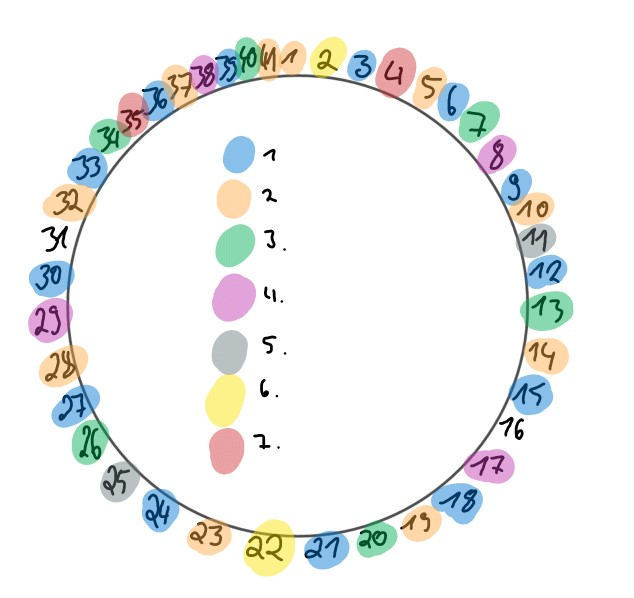
\includegraphics[width=7cm,height=7cm]{geogebra-export-1.jpg}\\
			\begin{multicols}{1}
			\noindent
			\textbf{Erste Runde}\\
			\noindent
			3 ist aus!\\
			6 ist aus!\\
			9 ist aus!\\
			12 ist aus!\\
			15 ist aus!\\
			18 ist aus!\\
			21 ist aus!\\
			24 ist aus!\\
			27 ist aus!\\
			30 ist aus!\\
			33 ist aus!\\
			36 ist aus!\\
			39 ist aus!\\
			\n
			\textbf{Zweite Runde}\\
			1 ist aus!\\
			5 ist aus!\\
			10 ist aus!\\
			14 ist aus!\\
			19 ist aus!\\
			23 ist aus!\\
			28 ist aus!\\
			32 ist aus!\\
			37 ist aus!\\
			41 ist aus!\\
			
			\noindent
			\textbf{Dritte Runde}\\
			7 ist aus!\\
			13 ist aus!\\
			20 ist aus!\\
			26 ist aus!\\
			34 ist aus!\\
			40 ist aus!\\
			\n
			\textbf{Vierte Runde}\\
			8 ist aus!\\
			17 ist aus!\\
			29 ist aus!\\
			38 ist aus!\\
			\n
			\textbf{Fünfte Runde}\\
			11 ist aus!\\
			25 ist aus!\\
			\n
			\textbf{Sechste Runde}\\
			2 ist aus!\\
			22 ist aus!\\
			\n
			\textbf{Siebte Runde}\\
			4 ist aus!\\
			35 ist aus!\\
			\n
			\underline{\underline{Person 16 und 31 überleben!}}
			\end{multicols}
			

		
			\endgroup
			
			\newpage
			\subsection*{b)}
			\begingroup
			\leftskip2em
			\begin{multicols}{3}

				\noindent
				\textbf{Erste Runde}\\
				\noindent
				10 ist aus!\\
				20 ist aus!\\
				30 ist aus!\\
				40 ist aus!\\
				\n
				\textbf{Zweite Runde}\\
				9 ist aus!\\
				21 ist aus!\\
				32 ist aus!\\
				\n
				\textbf{Dritte Runde}\\
				2 ist aus!\\
				14 ist aus!\\
				26 ist aus!\\
				38 ist aus!\\
				\n
				\textbf{Vierte Runde}\\
				11 ist aus!\\
				24 ist aus!\\
				37 ist aus!\\
				\n
				\columnbreak
				
				\noindent
				\textbf{Fünfte Runde}\\
				12 ist aus!\\
				27 ist aus!\\
				\n
				\textbf{Sechste Runde}\\
				1 ist aus!\\
				17 ist aus!\\
				34 ist aus!\\
				\n
				\textbf{Siebte Runde}\\
				8 ist aus!\\
				29 ist aus!\\
				\n
				
				
				\noindent
				\textbf{Achte Runde}\\
				6 ist aus!\\
				28 ist aus!\\
				\n
				\textbf{Neunte Runde}\\
				7 ist aus!\\
				33 ist aus!\\
				\n
				\textbf{Zehnte Runde}\\
				16 ist aus!\\
				41 ist aus!\\
				\n
				\textbf{Elfte Runde}\\
				25 ist aus!\\
				18 ist aus!\\
				\n
				\textbf{Zwölfte Runde}\\
				5 ist aus!\\
				3 ist aus!\\
				39 ist aus!\\
				\n
				\textbf{Dreizehnte Runde}\\
				4 ist aus!\\
				15 ist aus!\\
				23 ist aus!\\
				\n
				\textbf{Vierzehnte Runde}\\
				13 ist aus!\\
				36 ist aus!\\
				\n
				\textbf{Fünfzehnte Runde}\\\n
				22 ist aus!\\
				31 ist aus!\\
				\n
				\underline{\underline{Person 19 und 35 überleben!}}

			\end{multicols}
			\endgroup
		
		\section*{2.)}
		\begingroup
		\leftskip2em
		\begin{multicols}{3}
			
			\noindent
			\textbf{Erste Runde}\\ - 3 Personen aus\\
			\noindent
			10 ist aus!\\
			20 ist aus!\\
			30 ist aus!\\
			\n\textbf{Zweite Runde}\\ - 2 Personen aus\\
			11 ist aus!\\
			22 ist aus!\\
			\n\textbf{Dritte Runde}\\ - 3 Personen aus\\
			3 ist aus!\\
			15 ist aus!\\
			27 ist aus!\\
			\columnbreak
			
			\noindent
			\textbf{Vierte Runde}\\ - 2 Personen aus\\
			9 ist aus!\\
			24 ist aus!\\
			\n\textbf{Fünfte Runde}\\ - 2 Personen aus\\
			7 ist aus!\\
			23 ist aus!\\
			\n\textbf{Vierzehnte Runde}\\ - 2 Personen aus\\
			8 ist aus!\\
			26 ist aus!\\
			\n\textbf{Vierzehnte Runde}\\ - 1 Person aus\\
			14 ist aus!\\
			\columnbreak
			
			\noindent
			\textbf{Von nun an stehen nur noch 15 Personen} \\d.h. die Sicheren Positionen für die Gläubigen sind die folgenden:\\\n
			%\textit{\underline{2, 21, 16, 6, 4, 1, 5, 13, 19, 12, 29, 18, 25, 17, 28}} 
			\underline{\underline{1, 2, 4, 5, 6, 12, 13, 16, 17,}}\\\\
			\underline{\underline{18, 19, 21, 25, 28, 29!}}

		\end{multicols}
		\endgroup
		
		\newpage
		\section*{3.)}
		\begingroup
		\leftskip2em
		\subsection*{Rekursionsschema:}
			
			\begin{align*}
				J(1)&& &= &&1 &&a)\\
				J(2n)&& &= &&2*J(n)-1 &&b)\\
				J(2n+1)&& &= &&2*J(n)+1 &&c)	
			\end{align*}
		\endgroup
		
		\subsection*{a)}
			\begingroup
			\leftskip4em
			Es gilt zu zeigen, dass $\forall m \in \mathbb{N},\,m \ge 0 : J(2^m)=1$
			\subsubsection*{Induktionsanfang}
				$J(2^0)=1$
			\subsubsection*{Induktionsvoraussetzung}
				für $m=k \in \mathbb{N},\,k \,\ge 0 :$
				\begin{tabular}{lcc}
					$J(2^k)$ & $=$ & $1$ \\
				\end{tabular}
			\subsubsection*{Induktionsbehauptung}
				für $m=k+1 : J(2^{k+1})=1$
			\subsubsection*{Induktionsbeweis}

				\begin{align*}
					J(2^{k+1})&& &= && 1 \\
					J(2*2^k)&& &= && 1 && \text{| mit b) und }n=2^k\\
					2*J(2^k)-1&& &= && 1 && \text{| mit Induktionsvoraussetzung}\\
					2*1-1&& &= && 1 && &&\qedsymbol
				\end{align*}
			\endgroup
		
		\subsection*{b)}
			\begingroup
			\leftskip4em
			Es gilt zu zeigen, dass $\forall m \in \mathbb{N},\,m > 0 : J(2^m-1)=2^m-1$
			\subsubsection*{Induktionsanfang}
			
				\begin{tabular}{lccl}
					$J(2^1-1)$ & $=$ & $2^1-1$ & \\
					$J(1)$ & $=$ & $1$ & \\
				\end{tabular}
		
			\subsubsection*{Induktionsvoraussetzung}
				für $m=k \in \mathbb{N},\,k > 0 \, :$
				\begin{tabular}{lccl}
					$J(2^k-1)$ & $=$ & $2^k-1$ & \\
				\end{tabular}
			\subsubsection*{Induktionsbehauptung}
					$J(2^{k+1}-1)=2^{k+1}-1$ 
			\subsubsection*{Induktionsbeweis}
				\begin{align*}
					J(2^{k+1}-1-1+1)&& &= &&2^{k+1}-1 \\
					J(2^{k+1}-2+1)&& &= &&2^{k+1}-1 \\
					J(2*(2^k-1)+1)&& &= &&2^{k+1}-1 && \text{| mit c) und } n=(2^k-1)\\
					2*J(2^k-1)+1&& &= &&2^{k+1}-1 \\
					2*(2^k-1)+1&& &= &&2^{k+1}-1 \\
					2^{k+1}-1&& &= && 2^{k+1}-1 && &&\qed
				\end{align*}
			
			\endgroup	
			
		\subsection*{c)}
			\begingroup
			\leftskip4em
			Es gilt zu zeigen, dass $\forall m \in \mathbb{N},\,m \ge 0 : J(5*2^m)=2^{m+1}+1$
			\subsubsection*{Induktionsanfang}
				
				\begin{tabular}{lccl}
					$J(5*2^0)$ & $=$ & $2^{0+1}+1$ & \\
					$J(5)$ & $=$ & $3$ & \\
				\end{tabular}
			
			\subsubsection*{Induktionsvoraussetzung}
				für $m=k \in \mathbb{N},\,k \ge 0 \, :$
				\begin{tabular}{lcc}
					$J(5*2^k)$ & $=$ & $2^{k+1}+1$ \\
				\end{tabular}
			\subsubsection*{Induktionsbehauptung}
				für $m=k+1 : J(5*2^{k+1})=2^{k+2}+1$
			\subsubsection*{Induktionsbeweis}
				\begin{align*}
					J(5*2^{k+1})&& &= &&2^{k+2}+1 \\
					J(2*5*2^k)&& &= &&2^{k+2}+1 &&\text{| mit Rekursionsgleichung b) und } n = 5*2^k\\
					2*J(5*2^k)-1&& &= &&2^{k+2}+1 &&\text{| mit Induktionsvoraussetzung }\\
					2*(2^{k+1}+1)-1&& &= &&2^{k+2}+1 && &&\qedsymbol
				\end{align*}
			\endgroup
			
\end{document}